\graphicspath{ {HW-PIC/} }


\chapter{Hardware}

    \section{Umsetzung - V1}
    
    \subsection{V1}
        \subsubsection{Versorgung}
        Das Board wird mit 5V über USB-C versorgt, um den ESP32-S3 mit 3V3 zu 
        versorgung, wird ein AMS1117 Spannungswandler verwenden. Dieser wurde ausgewählt
        da das Gerät ohnehin mit dem Strometz verwendet wird. 
            \begin{figure}[h]
                \centering
                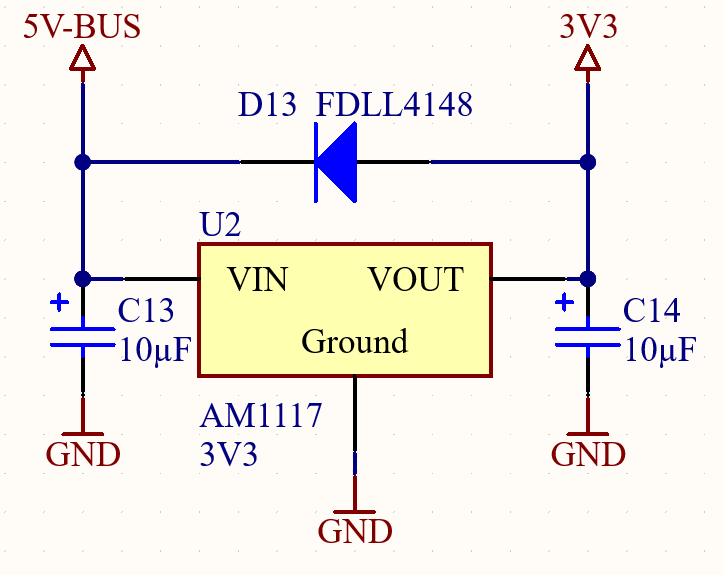
\includegraphics[width=8cm]{powersupply}
                \caption{AMS1117 mit 3V3 Ausgangsspannung.}
                \label{fig:sch1}
                
            \end{figure}

        Auf beiden Seiten einen Glättungskondensator. Die Diode wurde hinzugefügt um zu verhindern das am Ausgang eine größere Spannung
        anliegt als beim Eingang - wie z.B. beim Abstecken von dem Gerät.

        \newpage
        \subsubsection{Display}
        Das Display wird parralel im 8-BIT Modus angesteuert, die Pins mit denen 
        kommuniziert wird sind fix in der Libary festgelegt und können am Esp32-S3 
        frei auswählbar. 

            \begin{figure}[h!]
                \centering
                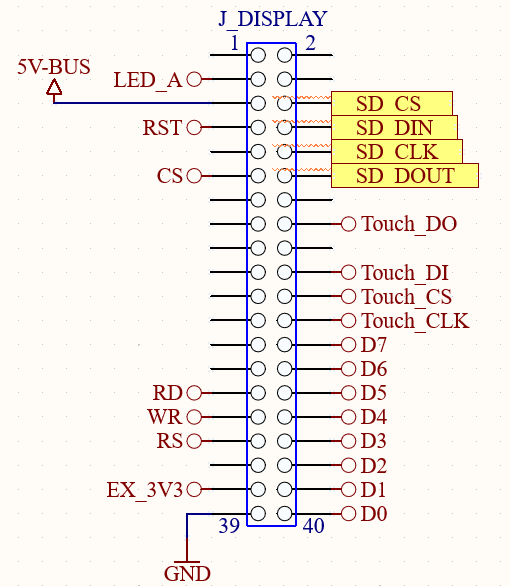
\includegraphics[width=8cm]{connector.png}
                \caption{Stecker für Display und Touch}
                \label{fig:sch2}

            \end{figure}

        Das zugekaufte Display hat ebenfalls ein SD-Kartenleser eingebaut, dieser wird 
        über SPI ausgelesen(Gelb markiert), ist aber für dieses Projekt nicht in der verwendung. 


        \subsubsection{Touch}
        Die Berührung am Resisivtouch-Panel wird vom XPT2046 erfasst und mittels 
        SPI-BUS vom µC ausgelesen. Da es bei der Implementierung von Touch softwareseitig
        Probleme gab, wurde sich für eine Eingabe mit einem Rotary Encoder entschieden.
        Dafür wurden die in der Abbildung \ref{fig:sch2} gezeigten Pins mit dem prefix "Touch" 
        für das Einlesen des Drehgebers verwendet.
